\documentclass{beamer}

\usetheme{Warsaw}
%\usetheme{CambridgeUS}

% modification history
% created on 18 sep 2011
% modified on 25 mar

%\usepackage{amsfonts, amsmath, amssymb}

%\setbeamertemplate{theorems}[numbered]
%\setbeamertemplate{theorems}[ams style] 
\usepackage[skins,breakable]{tcolorbox}
%\usepackage[normalem]{ulem}

%\usefonttheme[onlymath]{serif}                     // change the style of math font 

%=============set slide number=================
\addtobeamertemplate{navigation symbols}{}{
    \usebeamerfont{footline}
    \usebeamercolor[fg]{footline}
    \hspace{1em}
    \insertframenumber/\inserttotalframenumber
}
\setbeamercolor{footline}{fg=black}
\setbeamerfont{footline}{series=\bfseries}


%=============set footline=====================
\setbeamertemplate{footline}
{
  \leavevmode%
  \hbox{%
  \begin{beamercolorbox}[wd=.55\paperwidth,ht=2.25ex,dp=1ex,center]{author in head/foot}%
    \usebeamerfont{author in head/foot}\insertshortauthor
  \end{beamercolorbox}%
  \begin{beamercolorbox}[wd=.45\paperwidth,ht=2.25ex,dp=1ex,center]{title in head/foot}%
    \usebeamerfont{title in head/foot}\insertshorttitle
  \end{beamercolorbox}}%
  \vskip0pt%
}

%creating a rectangle box def
\newtcbox{\mybox}[1][red]{arc=0pt,outer arc=0pt,colback=#1!10!white,colframe=#1!50!black, boxsep=0pt,left=1pt,right=1pt,top=2pt,bottom=2pt,boxrule=0pt,bottomrule=1pt,toprule=1pt}

\newtcbox{\xmybox}[1][red]{arc=7pt,colback=#1!10!white,colframe=#1!50!black,before upper={\rule[-3pt]{0pt}{10pt}},boxrule=1pt,boxsep=0pt,left=6pt,right=6pt,top=2pt,bottom=2pt}
%the ``on line'' option doesn't work. so omitting it

%===== spacing =====

\def\extraspacing{\vspace{2mm} \noindent}
\def\vgap{\vspace{2mm}}
\def\hgap{\textrm{\hspace{1mm}}}

%===== tabbing =====

\def\tab{\hspace{2mm}}
\def\tabpos{\hspace{4mm} \= \hspace{4mm} \= \hspace{4mm} \= \hspace{4mm} \=
\hspace{4mm} \= \hspace{4mm} \= \hspace{4mm} \= \hspace{4mm} \= \hspace{4mm}
\kill}
\newcommand{\mytab}[1]{\begin{tabbing}\tabpos #1\end{tabbing}}

%===== blocks =====

% \newtheorem{theorem}{Theorem}
% \newtheorem{lemma}{Lemma}
% \newtheorem{corollary}{Corollary}
% \newtheorem{proposition}{Proposition}
% \newtheorem{definition}{Definition}
% \newtheorem{problem}{Problem}

\newcommand{\cbox}[2]{\begin{tcolorbox}[arc=0mm, colframe=#1!50!black, colback=#1!10!white]#2\end{tcolorbox}}
\newcommand{\minipg}[2]{\begin{center}\begin{minipage}{#1}#2\end{minipage}\end{center}}
\newcommand{\myfrm}[1]{\begin{frame}\begin{small}#1\end{small}\end{frame}} 
\newcommand{\myitems}[1]{\begin{itemize}#1\end{itemize}}
\newcommand{\myenums}[1]{\begin{enumerate}#1\end{enumerate}}
\newcommand{\myfig}[1]{\begin{figure}\centering #1\end{figure}}
    
%===== math macros =====
\newcommand{\bm}[1]{\textrm{\boldmath${#1}$}}
%\newcommand{\smat}[2]{\left[\begin{tabular}{#1}#2\end{tabular}\right]}
%\newcommand{\bmat}[2]{\left|\begin{tabular}{#1}#2\end{tabular}\right|}
\newcommand{\bmat}[1]{\begin{bmatrix}#1\end{bmatrix}}
\newcommand{\vmat}[1]{\begin{vmatrix}#1\end{vmatrix}}
\newcommand{\myeqn}[1]{\begin{eqnarray}#1\end{eqnarray}}
\newcommand{\set}[1]{\{#1\}}

\def\eps{\epsilon}
\def\fr{\frac}
\def\lc{\lceil}
\def\lf{\lfloor}
\def\rc{\rceil}
\def\rf{\rfloor}
\def\Pr{\textrm{\boldmath$Pr$}}
\def\expt{\textrm{\boldmath$E$}}
\def\real{\mathbb{R}}
\def\int{\mathbb{Z}}
\def\*{\star}
\def\tO{\tilde{O}}

\DeclareMathOperator*{\argmin}{arg\,min}
\DeclareMathOperator*{\polylg}{polylg}
\DeclareMathOperator*{\polylog}{polylog}
\DeclareMathOperator*{\intr}{\cap}

\def\nn{\nonumber}
\def\mit{\mathit}


%===== misc =====

\def\done{\hspace*{\fill} $\framebox[2mm]{}$}	% end of proof
\def\ttt{\texttt}

%===== coloring =====
\newcommand{\red}[1]{\textcolor{red}{#1}}
\newcommand{\bred}[1]{\textcolor{red}{\bf #1}}
\newcommand{\blue}[1]{\textcolor{blue}{\bf #1}}

\usepackage{color}
\usepackage{graphicx}
\usepackage{multirow}
\usepackage{wrapfig}
\usepackage[skins,breakable]{tcolorbox}

\def\done{\hfill$\square$}
\def\ttt{\texttt}
\def\vgap{\vspace{5mm}}

\def\sort{\mit{sort}}

\title[DATABASE SYSTEM PRINCIPLES]{Query Processing 4:\\ Hash Join}

\author[Yufei Tao @ NTU]{Yufei Tao}
\institute[]{\url{https://www.cse.cuhk.edu.hk/~taoyf}}
\date{}

% \def\dtm{\mathit{d\mbox{-}tm}}
% \def\ftm{\mathit{f\mbox{-}tm}}
\def\bestext{\mathit{best\mbox{-}ext}}

\begin{document}
%-------------------------------------------------------------
\begin{frame}
    \titlepage
%     \begin{tcolorbox}[arc=0mm, colframe=green!50!black, colback=green!10!white] 
%     \end{tcolorbox}
\end{frame}
%-------------------------------------------------------------
\begin{frame}
\begin{small}
    This lecture will introduce the \blue{hash join} algorithm for computing a natural join involving two relations.
    %\vgap
\end{small}    
\end{frame}
%-------------------------------------------------------------
\myfrm{
    \xmybox{The Binary Join Problem}

    \vgap

    $\red{R_1(X, Y)}$: A relation with attributes $X$ and $Y$. \\
    $\red{R_2(X, Z)}$: A relation with attributes $X$ and $Z$. \\
    $\red{B_1} =$ the number of disk blocks that $R_1$ occupies. \\
    $\red{B_2} =$ the number of disk blocks that $R_2$ occupies. \\
    $\red{M} =$ the number of memory blocks (a.k.a., the buffer blocks). \\
    \myitems{
        \item We assume that $M \ge 7$ and $M - 1$ is a multiple of 3.
    }

    \vgap

    \blue{Goal:} Compute the join result $R_1 \bowtie R_2$.

    \vgap

    \cbox{blue}{
        Recall that the \blue{block-based nested loop} (BNL) algorithm can compute the join result in $\red{B_1 + \lc \fr{B_1}{M-1} \rc B_2}$ I/Os. In particular, if $R_1$ can be loaded into memory entirely, then the I/O cost of BNL is $B_1 + B_2$.
    }

}
%-------------------------------------------------------------
\myfrm{
    \xmybox{Hashing}

    \vgap

    Let $\red{\mathbb{D}}$ be the domain of the ``join attribute'' $X$. Set
    \myeqn{
        \red{U} = (M-1)/3 \nn
    }
    We are given a \blue{hash function} $\red{H}$, which is a function mapping $\mathbb{D}$ to the set of integers $\set{1, 2, ..., U}$.


    \vgap

    Given a tuple $\red{t_1}$ of $R_1$, we refer to $H(t_1.X)$ as the \blue{hash value} of $t_1$. \\
    Given a tuple $\red{t_2}$ of $R_2$, we refer to $H(t_2.X)$ as the \blue{hash value} of $t_2$.


    \vgap

    We will carry out our discussion under the following assumption:

    \cbox{blue}{
        \blue{Good hashing assumption:} For any $\red{h} \in [1, U]$, the tuples of $R_1$ with hash value $h$ can fit in $\red{U}$ blocks.
    }

    No such requirements are placed on $R_2$.
}
%-------------------------------------------------------------
\myfrm{
    \xmybox{Buckets}

    %\vgap

    Given a value $\red{h} \in [1, U]$, define
    \myeqn{
        \red{R_1(h)} &=& \set{ \text{tuple $t \in R_1$} \mid H(t_1.X) = h} \nn \\
        \red{R_2(h)} &=& \set{ \text{tuple $t \in R_2$} \mid H(t_2.X) = h} \nn
    }
    We will refer to $R_1(h)$ and $R_2(h)$ as \blue{buckets}. Clearly, each relation has $U$ buckets.

    \vgap

    \cbox{blue}{
        \blue{Fact:} $R_1 \bowtie R_2 = \bigcup_{h=1}^U R_1(h) \bowtie R_2(h)$.
    }

    In other words, once we have obtained all buckets, we can focus on joining each $R_1(h)$ with the \bred{corresponding} $R_2(h)$.

}
%-------------------------------------------------------------
\myfrm{
    \xmybox{Hash Join}

    \vgap

    \blue{Step 1:} Create the $U$ buckets of $R_1$ and $R_2$, respectively. \\
    \blue{Step 2:} For each $\red{h} \in [1, U]$, compute $R_1(h) \bowtie R_2(h)$.

    \vgap

    We will discuss each step in turn.
}
%-------------------------------------------------------------
\myfrm{
    \xmybox{Hash Join: Step 1}

    \vgap

    We will explain how to create the $U$ buckets of $R_1$.
    %A similar algorithm works for $R_2$.

    \vgap

    Use one memory block as the \blue{output buffer} for each bucket $\red{R_1(h)}$, where $h \in [1, U]$. \\ %This needs $U \le M-1$ blocks. \\
    Use one memory block as the \blue{input buffer} for reading $R_1$.


}
%-------------------------------------------------------------
\myfrm{
    \xmybox{Hash Join: Step 1}

    For each tuple $\red{t}$ read from $R_1$, add it to the output buffer of $R_1(H(t.X))$.

    \vgap

    When an output buffer --- say for bucket $\red{R_1(h)}$ of some $h \in [1, U]$ --- is \bred{full}, append it to the file of $R_1(h)$ on disk.

    \cbox{green}{
    \blue{Example:} $U = 2$ and $H(x) = 1 + (x \text{ mod } 2)$.

    \begin{center}
        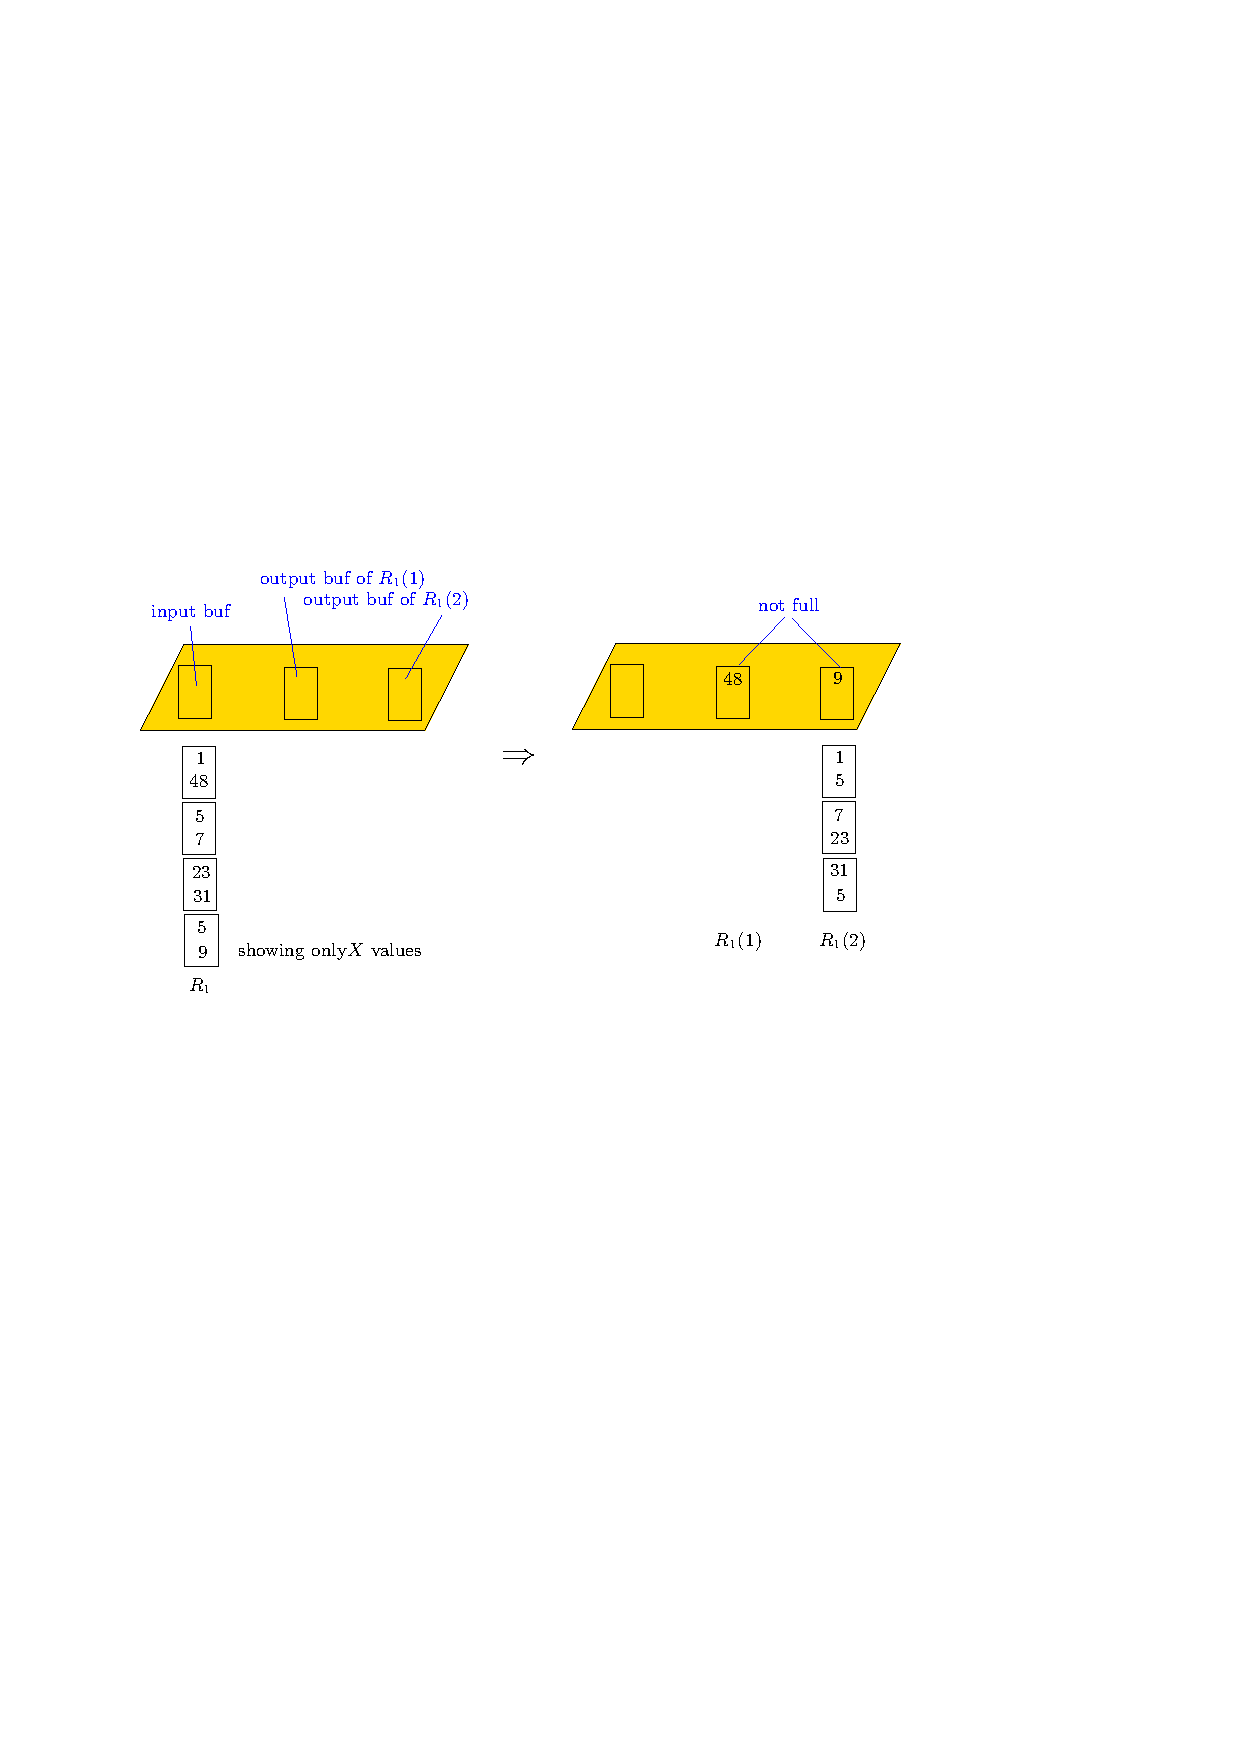
\includegraphics[height=40mm]{./artwork/hj1}
    \end{center}
    }

}
%-------------------------------------------------------------
\myfrm{
    \xmybox{Hash Join: Step 1}

    The I/O cost is bounded by $\red{2B_1}$ because
    \myitems{
        \item every block of $R_1$ is read once;
        \item the number of full blocks flushed to the disk is at most $B_1$.
    }

    \begin{center}
        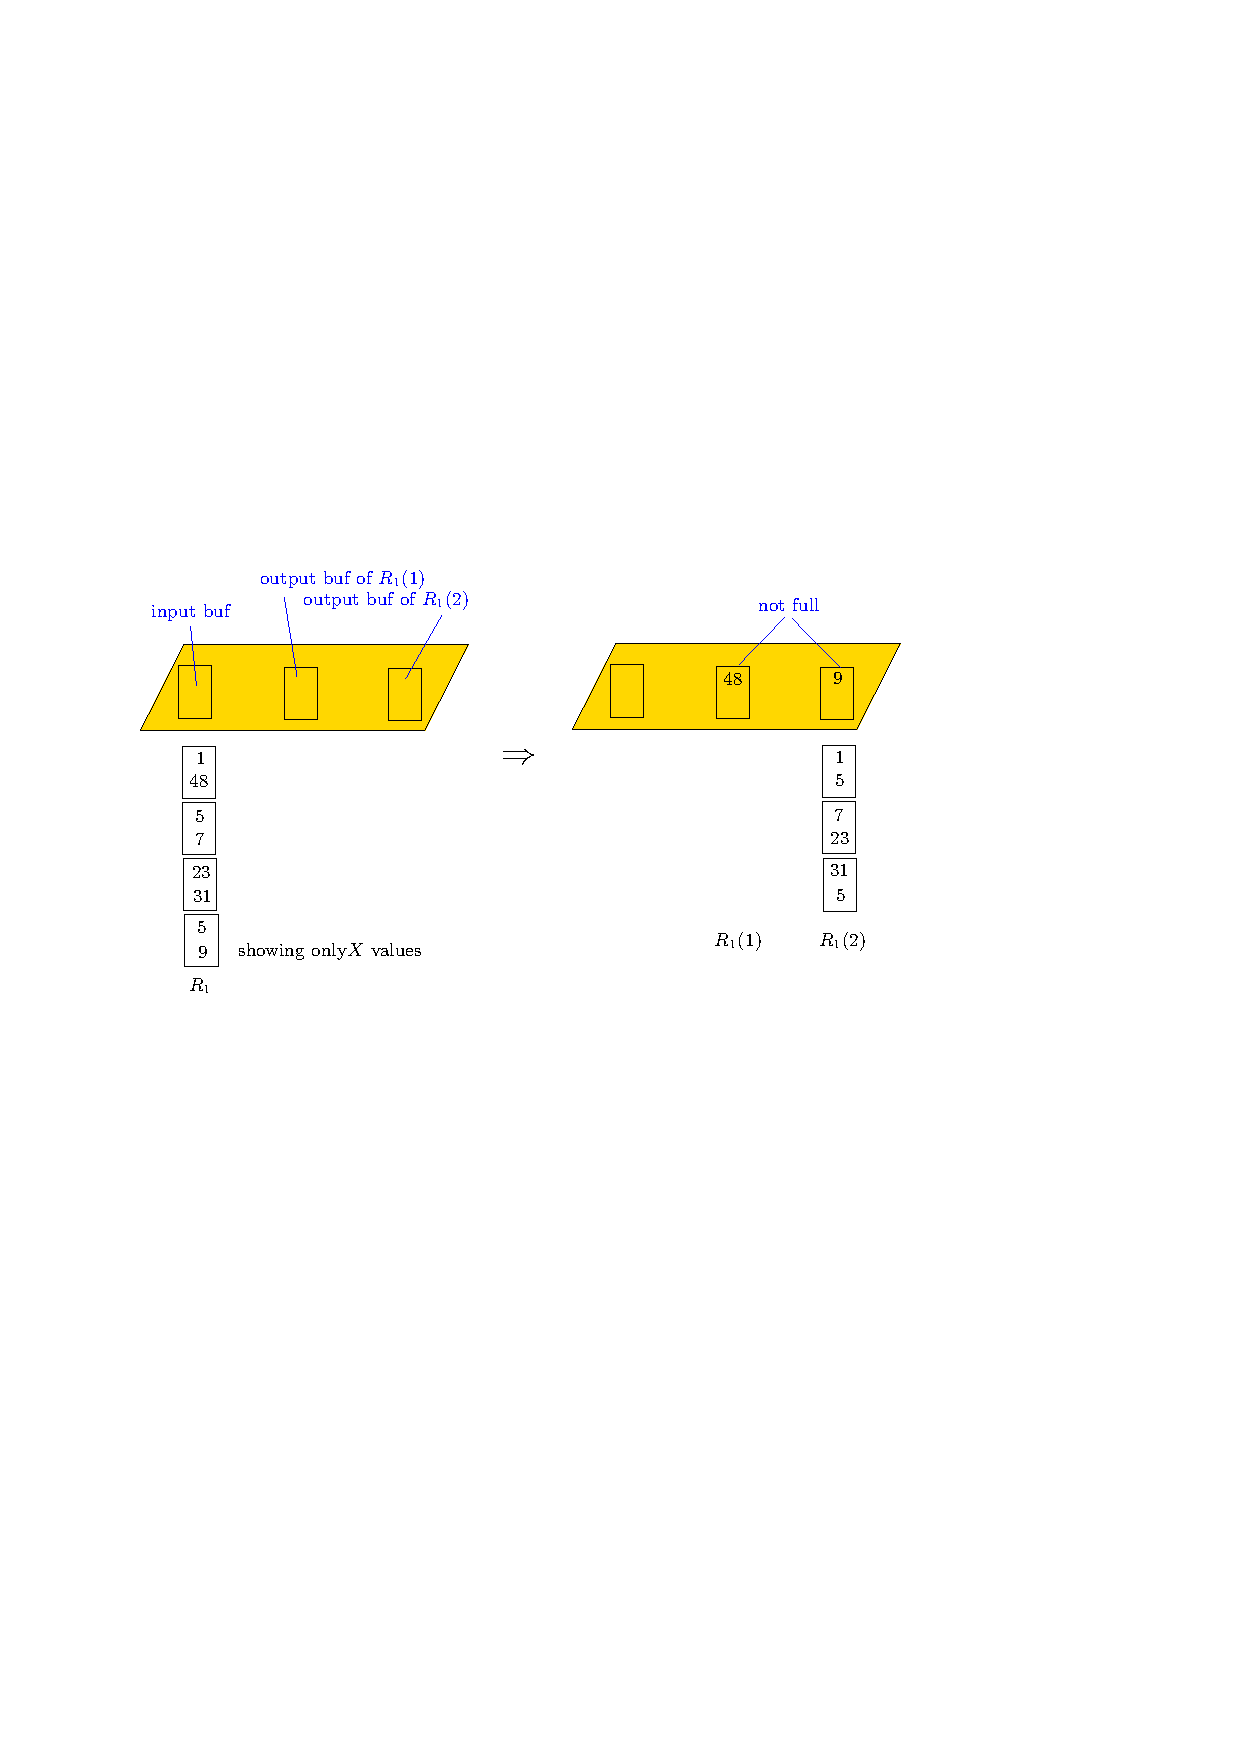
\includegraphics[height=35mm]{./artwork/hj1}
    \end{center}

    \cbox{blue}{
        \blue{Remark:} Each bucket can have \bred{at most one non-full block}, and this block \bred{must reside in memory}. We do not write those blocks to disk; otherwise, the I/O cost can increase to $2B_1 + U$ in the worst case (\blue{think:} why?).
    }
}
%-------------------------------------------------------------
\myfrm{
    \xmybox{Hash Join: Step 1}

    \vgap

    Create the $U$ buckets of $R_2$ in the same way, while keeping the non-full bucket blocks of $R_1$ in memory.

    \vgap

    The I/O cost is bounded by $\red{2B_2}$

    \vgap

    At this moment, we have used $2U$ memory blocks:
    \myitems{
        \item $U$ blocks for $R_1$ (each may be the non-full block of a bucket);
        \item $U$ blocks for $R_2$ (each may be the non-full block of a bucket).
    }
}
%-------------------------------------------------------------
\myfrm{
    \xmybox{Hash Join: Step 2}

    \vgap

    \blue{Step 2:} For each $\red{h} \in [1, U]$, compute $R_1(h) \bowtie R_2(h)$.

    \vgap



    %\vgap

    Apply BNL to compute $R_1(h) \bowtie R_2(h)$. By the good hashing assumption, $R_1(h)$ can be loaded into $U$ memory blocks. Then, use one memory block to scan $R_2(h)$.
    \myitems{
        \item In total, we use at most $3U + 1 = M$ memory blocks.
    }

    \vgap

    The I/O cost is bounded by $\red{B_1 + B_2}$ because every disk-resident block of the $2U$ buckets is read exactly once.
}
%-------------------------------------------------------------
\myfrm{
    \cbox{blue}{
        Overall, the hash join algorithm performs $3(B_1 + B_2)$ I/Os.
    }

    \vgap

    \cbox{red}{
        \blue{Remark.} Recall that our analysis requires the good hashing assumption. \bred{This assumption may not hold when data are ``skewed''.} For example, if all the tuples of $R_1(X, Y)$ share the same $X$-value, no hash function can satisfy the assumption as long as $B_1 > U$. In the presence of data skew, hash join can be prohibitively expensive.
    }
}
%-------------------------------------------------------------

\end{document} 


